\subsection{Problem}

\renewcommand{\theequation}{\theenumi}
\begin{enumerate}[label=\thesection.\arabic*.,ref=\thesection.\theenumi]
\numberwithin{equation}{enumi}
	\item A doctor is to visit a patient. From the past experience, it is known that the probabilities that he will come by train, bus, scooter or by other means of transport are respectively $\frac{3}{10},\frac{1}{5},\frac{1}{10},\frac{2}{5}$. The probabilities that he will be late are $\frac{1}{4},\frac{1}{3},\frac{1}{12}$ , if he comes by train, bus and scooter respectively, but if he4 comes by other means of transport, then he will not be late. When he arrives, he is late.What is the probability that he comes by train?
\\
\solution Let $T_1,T_2,T_3,T_4$ denote the events where the doctor came by train,bus,scooter and other means of transport. Let L denote the event that the doctor arrives late. We need to find the probability that the doctor comes by train if he's late.i.e.$P\brak{\frac{T_1}{L}}$.
\\
\begin{align}
P\brak{T_1} = \frac{3}{10} \quad  P\brak{T_2} = \frac{1}{5} \quad  P\brak{T_3}  = \frac{1}{10} \quad P\brak{T_4} = \frac{2}{5}
\end{align}


\begin{align}
P\brak{\frac{L}{T_1}} &= P\brak{\text{Arrives late coming by train}}\\
P\brak{\frac{L}{T_1}} &= \frac{1}{4}
\end{align}

\begin{align}
P\brak{\frac{L}{T_2}} &= P\brak{\text{Arrives late coming by bus}}\\
P\brak{\frac{L}{T_2}} &= \frac{1}{3}
\end{align}
\begin{align}
P\brak{\frac{L}{T_3}} &= P\brak{\text{Arrives late coming by scooter}}\\
P\brak{\frac{L}{T_3}} &= \frac{1}{12}
\end{align}

\begin{align}
P\brak{\frac{L}{T_4}} &= P\brak{\text{Arrives late coming by other means}}\\
P\brak{\frac{L}{T_4}} &= 0
\end{align}


\begin{multline}
P\brak{\frac{T_1}{L}} =\\ \frac{P\brak{T_1}.P\brak{\frac{L}{T_1}}}{P\brak{T_1}.P\brak{\frac{L}{T_1}} + P\brak{T_2}.P\brak{\frac{L}{T_2}}  + P\brak{T_3}.P\brak{\frac{L}{T_3}} +P\brak{T_4}.P\brak{\frac{L}{T_4}} }
\end{multline}
\begin{align}
P\brak{\frac{T_1}{L}} &= \frac{\frac{3}{40}}{\frac{18}{120}}
\end{align}
which is calculated to be 0.5






\begin{comment}	
	The following python code computes the value of x and y used in Fig.\ref{fig:qten}.
	\begin{lstlisting}
	./codes/lines/q10.py
	\end{lstlisting}
	
	\solution In a parallelogram, the diagonals bisect each other. Hence
	\begin{align}
		\vec{\frac{A+C}{2} = \frac{B+L}{2}}
		\\
\therefore \vec{\frac{1+x}{2} = \frac{7}{2}}\text{ and }\vec{\frac{8}{2} = \frac{y+5}{2}} \\
\implies x=6,y=3
\end{align}
	\begin{figure}[!ht]
	\centering
	\includegraphics[width=\columnwidth]{./figs/lines/q10.eps}
	\caption{Parallelogram of Q.3.6.5}
	\label{fig:qten}	
	\end{figure}
\end{comment}	
		
\end{enumerate}
